\documentclass[12pt,letterpaper]{article}
\usepackage{graphicx,textcomp}
\usepackage{natbib}
\usepackage{setspace}
\usepackage{fullpage}
\usepackage{color}
\usepackage[reqno]{amsmath}
\usepackage{amsthm}
\usepackage{fancyvrb}
\usepackage{amssymb,enumerate}
\usepackage[all]{xy}
\usepackage{endnotes}
\usepackage{lscape}
\newtheorem{com}{Comment}
\usepackage{float}
\usepackage{hyperref}
\newtheorem{lem} {Lemma}
\newtheorem{prop}{Proposition}
\newtheorem{thm}{Theorem}
\newtheorem{defn}{Definition}
\newtheorem{cor}{Corollary}
\newtheorem{obs}{Observation}
\usepackage[compact]{titlesec}
\usepackage{dcolumn}
\usepackage{tikz}
\usetikzlibrary{arrows}
\usepackage{multirow}
\usepackage{xcolor}
\newcolumntype{.}{D{.}{.}{-1}}
\newcolumntype{d}[1]{D{.}{.}{#1}}
\definecolor{light-gray}{gray}{0.65}
\usepackage{url}
\usepackage{listings}
\usepackage{color}

\definecolor{codegreen}{rgb}{0,0.6,0}
\definecolor{codegray}{rgb}{0.5,0.5,0.5}
\definecolor{codepurple}{rgb}{0.58,0,0.82}
\definecolor{backcolour}{rgb}{0.95,0.95,0.92}

\lstdefinestyle{mystyle}{
	backgroundcolor=\color{backcolour},   
	commentstyle=\color{codegreen},
	keywordstyle=\color{magenta},
	numberstyle=\tiny\color{codegray},
	stringstyle=\color{codepurple},
	basicstyle=\footnotesize,
	breakatwhitespace=false,         
	breaklines=true,                 
	captionpos=b,                    
	keepspaces=true,                 
	numbers=left,                    
	numbersep=5pt,                  
	showspaces=false,                
	showstringspaces=false,
	showtabs=false,                  
	tabsize=2
}
\lstset{style=mystyle}
\newcommand{\Sref}[1]{Section~\ref{#1}}
\newtheorem{hyp}{Hypothesis}


\title{Problem Set 4}
\date{Qin Guo 24338859}
\author{Applied Stats/Quant Methods 1}


\begin{document}
	\maketitle
	\section*{Instructions}
	\begin{itemize}
		\item Please show your work! You may lose points by simply writing in the answer. If the problem requires you to execute commands in \texttt{R}, please include the code you used to get your answers. Please also include the \texttt{.R} file that contains your code. If you are not sure if work needs to be shown for a particular problem, please ask.
		\item Your homework should be submitted electronically on GitHub.
		\item This problem set is due before 23:59 on Monday November 18, 2024. No late assignments will be accepted.
	\end{itemize}



	\vspace{.5cm}
\section*{Question 1: Economics}
\vspace{.25cm}
\noindent 	
In this question, use the \texttt{prestige} dataset in the \texttt{car} library. First, run the following commands:

\begin{verbatim}
install.packages(car)
library(car)
data(Prestige)
help(Prestige)
\end{verbatim} 


\noindent We would like to study whether individuals with higher levels of income have more prestigious jobs. Moreover, we would like to study whether professionals have more prestigious jobs than blue and white collar workers.

\newpage
\begin{enumerate}
	
	\item [(a)]
	Create a new variable \texttt{professional} by recoding the variable \texttt{type} so that professionals are coded as $1$, and blue and white collar workers are coded as $0$ (Hint: \texttt{ifelse}).
		\lstinputlisting[language=R, firstline=2, lastline=11]{PS04_Qin Guo.R}
	\vspace{2cm}
	
	
	\item [(b)]
	Run a linear model with \texttt{prestige} as an outcome and \texttt{income}, \texttt{professional}, and the interaction of the two as predictors (Note: this is a continuous $\times$ dummy interaction.)
		\lstinputlisting[language=R, firstline=13, lastline=17]{PS04_Qin Guo.R}
		\begin{figure}[h]
			\centering
			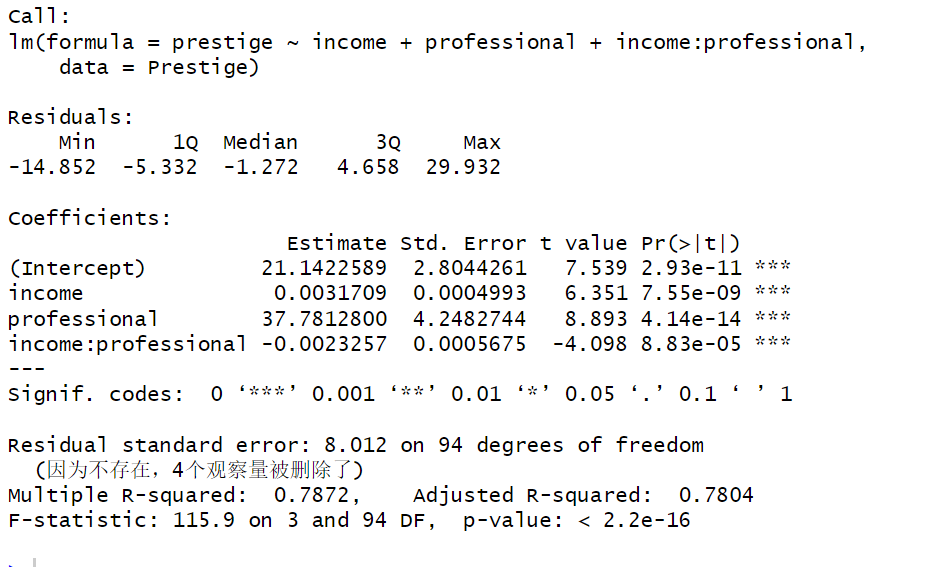
\includegraphics[width=0.8\textwidth]{Question1_data.png}
		\end{figure}	
	\vspace{6cm}
	\item [(c)]
	Write the prediction equation based on the result.
			\begin{align*}
			Prestige = 21.142 + 0.003*Income + 37.781*Professional -\\ 0.002*Income*Professional \times \text{difflog}
		\end{align*}
	\item [(d)]
	Interpret the coefficient for \texttt{income}.\\
	When other variables are controlled, especially when the professional variable is 0, the average change in prestige (prestige score) for each unit increase in income is 0.For blue-collar and white-collar workers, the average change in prestige (prestige score) for each unit increase in income is 0.003 units. 	
	\item [(e)]
	Interpret the coefficient for \texttt{professional}.\\
	The coefficient of professional indicates the average change in prestige when changing from a non-professional(blue-collar or white-collar workers) to a professional, while controlling for other variables (such as income).The average prestige score of professional worker is about 37.781 units higher than an equally income blue-collar or white-collar worker.

	\item [(f)]
	What is the effect of a \$1,000 increase in income on prestige score for professional occupations? In other words, we are interested in the marginal effect of income when the variable \texttt{professional} takes the value of $1$. Calculate the change in $\hat{y}$ associated with a \$1,000 increase in income based on your answer for (c).
	\lstinputlisting[language=R, firstline=19, lastline=30]{PS04_Qin Guo.R}
		\begin{figure}[h]
		\centering
		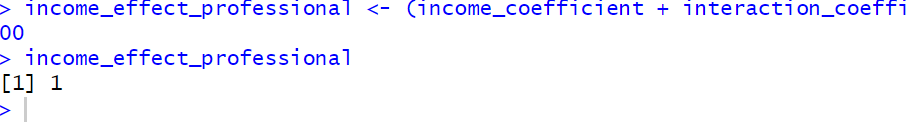
\includegraphics[width=0.8\textwidth]{Question1_f.png}
	\end{figure}\\
		According to the result, there is only a 1 prestige point difference for a 
	    1000dollars increase in income for professional occupations.
	    
	\vspace{10cm}
	
	
	\item [(g)]
	What is the effect of changing one's occupations from non-professional to professional when her income is \$6,000? We are interested in the marginal effect of professional jobs when the variable \texttt{income} takes the value of $6,000$. Calculate the change in $\hat{y}$ based on your answer for (c).
	\lstinputlisting[language=R, firstline=32, lastline=36]{PS04_Qin Guo.R}
	\begin{figure}[h]
		\centering
		
\includegraphics[width=0.8\textwidth]{Question1_g.png}
	\end{figure}\\
	According to the result, it shows that there would be a predicted 25.781 increase in prestige score from non-professional to professional when her income is 6000dollars. 
	
\end{enumerate}
	\vspace{3cm}

\section*{Question 2: Political Science}
\vspace{.25cm}
\noindent 	Researchers are interested in learning the effect of all of those yard signs on voting preferences.\footnote{Donald P. Green, Jonathan	S. Krasno, Alexander Coppock, Benjamin D. Farrer,	Brandon Lenoir, Joshua N. Zingher. 2016. ``The effects of lawn signs on vote outcomes: Results from four randomized field experiments.'' Electoral Studies 41: 143-150. } Working with a campaign in Fairfax County, Virginia, 131 precincts were randomly divided into a treatment and control group. In 30 precincts, signs were posted around the precinct that read, ``For Sale: Terry McAuliffe. Don't Sellout Virgina on November 5.'' \\

Below is the result of a regression with two variables and a constant.  The dependent variable is the proportion of the vote that went to McAuliff's opponent Ken Cuccinelli. The first variable indicates whether a precinct was randomly assigned to have the sign against McAuliffe posted. The second variable indicates
a precinct that was adjacent to a precinct in the treatment group (since people in those precincts might be exposed to the signs).  \\

\vspace{.5cm}
\begin{table}[!htbp]
	\centering 
	\textbf{Impact of lawn signs on vote share}\\
	\begin{tabular}{@{\extracolsep{5pt}}lccc} 
		\\[-1.8ex] 
		\hline \\[-1.8ex]
		Precinct assigned lawn signs  (n=30)  & 0.042\\
		& (0.016) \\
		Precinct adjacent to lawn signs (n=76) & 0.042 \\
		&  (0.013) \\
		Constant  & 0.302\\
		& (0.011)
		\\
		\hline \\
	\end{tabular}\\
	\footnotesize{\textit{Notes:} $R^2$=0.094, N=131}
\end{table}

\vspace{.5cm}
\begin{enumerate}
	\item [(a)] Use the results from a linear regression to determine whether having these yard signs in a precinct affects vote share (e.g., conduct a hypothesis test with $\alpha = .05$).
		\lstinputlisting[language=R, firstline=39, lastline=50]{PS04_Qin Guo.R}\\
		Null Hypothesis: The presence of yard signs has no effect on the vote share.\\
		                     H0:$\beta = 0$\\
		Alternative Hypothesis: The presence of yard signs has an effect on the vote share.\\
				             Ha:$\beta \neq 0$
				             \vspace{0.5cm}
	 \\Conclusion: P-value of 0.0097 is less than 0.05, therefore, we reject the null hypothesis. So there is a significant effect of yard signs on the vote share.
	\item [(b)]  Use the results to determine whether being
	next to precincts with these yard signs affects vote
	share (e.g., conduct a hypothesis test with $\alpha = .05$).\\
	\lstinputlisting[language=R, firstline=51, lastline=60]{PS04_Qin Guo.R}\\
		Null Hypothesis: being next to precincts with these yard signs does not effect on the vote share.\\
	H0:$\beta = 0$\\
	Alternative Hypothesis: being next to precincts with these yard signs effects on the vote share.\\
	Ha:$\beta \neq 0$
	\vspace{0.5cm}
	\\Conclusion: P-value of 0.00157 is less than 0.05, therefore, we reject the null hypothesis. So there is a significant effect of being next to precincts with yard signs on the vote share.
	\vspace{1cm}
	\item [(c)] Interpret the coefficient for the constant term substantively.\\
	The constant term coefficient of 0.302 signifies the average proportion of votes that Ken Cuccinelli, McAuliffe's opponent, would receive in precincts where no lawn signs were installed and which are not in proximity to any precincts with such signs.\\
	
	
	
	\vspace{1cm}
	
	\item [(d)] Evaluate the model fit for this regression.  What does this	tell us about the importance of yard signs versus other factors that are not modeled?\\
	An R-squared value of 0.094 indicates that the influence of yard signs accounted for only 9.4 \% of the vote share. This suggests that while yard signs might have some impact, they are not strong predictors of voting behavior.\\
	
	
	
	
	
	
\end{enumerate}  


\end{document}
